\documentclass[10pt,twocolumn]{article}
\usepackage[a4paper,margin=2cm,columnsep=0.7cm]{geometry}
\usepackage[T1]{fontenc}
\usepackage[utf8]{inputenc}
\usepackage{lmodern}
\usepackage{microtype}
\usepackage{amsmath,amssymb}
\usepackage{graphicx}
\usepackage{booktabs}
\usepackage{enumitem}
\usepackage{xspace}
\usepackage[numbers,sort&compress]{natbib}
\usepackage[font=small,labelfont=bf]{caption}
\usepackage{xcolor}
\usepackage[colorlinks=true,linkcolor=black,citecolor=black,urlcolor=blue!50!black]{hyperref}
\usepackage{url}

% generated by src/make_numbers.py -- do not edit
\newcommand{\AICMetrics}{88.4\xspace}
\newcommand{\AICMetricsLevel}{87.0\xspace}
\newcommand{\BankFutoshikiClues}{10.1\xspace}
\newcommand{\BankFutoshikiLA}{0\xspace}
\newcommand{\BankFutoshikiLB}{619\xspace}
\newcommand{\BankFutoshikiLC}{881\xspace}
\newcommand{\BankFutoshikiLD}{0\xspace}
\newcommand{\BankFutoshikiLE}{0\xspace}
\newcommand{\BankKillerClues}{8.4\xspace}
\newcommand{\BankKillerLA}{0\xspace}
\newcommand{\BankKillerLB}{582\xspace}
\newcommand{\BankKillerLC}{600\xspace}
\newcommand{\BankKillerLD}{314\xspace}
\newcommand{\BankKillerLE}{4\xspace}
\newcommand{\BankSudokuClues}{24.3\xspace}
\newcommand{\BankSudokuLA}{738\xspace}
\newcommand{\BankSudokuLB}{214\xspace}
\newcommand{\BankSudokuLC}{548\xspace}
\newcommand{\BankSudokuLD}{0\xspace}
\newcommand{\BankSudokuLE}{0\xspace}
\newcommand{\BankSudokuXClues}{24.3\xspace}
\newcommand{\BankSudokuXLA}{3{,}859\xspace}
\newcommand{\BankSudokuXLB}{1{,}110\xspace}
\newcommand{\BankSudokuXLC}{3{,}031\xspace}
\newcommand{\BankSudokuXLD}{0\xspace}
\newcommand{\BankSudokuXLE}{0\xspace}
\newcommand{\BankZebraClues}{13.6\xspace}
\newcommand{\BankZebraHardClues}{13.2\xspace}
\newcommand{\BankZebraHardLA}{0\xspace}
\newcommand{\BankZebraHardLB}{57\xspace}
\newcommand{\BankZebraHardLC}{198\xspace}
\newcommand{\BankZebraHardLD}{45\xspace}
\newcommand{\BankZebraHardLE}{0\xspace}
\newcommand{\BankZebraLA}{0\xspace}
\newcommand{\BankZebraLB}{360\xspace}
\newcommand{\BankZebraLC}{967\xspace}
\newcommand{\BankZebraLD}{173\xspace}
\newcommand{\BankZebraLE}{0\xspace}
\newcommand{\CallsEFive}{4\xspace}
\newcommand{\CallsEFour}{35\xspace}
\newcommand{\CallsEOne}{100\xspace}
\newcommand{\CallsEThree}{75\xspace}
\newcommand{\CallsETwo}{20\xspace}
\newcommand{\CallsHaiku}{81\xspace}
\newcommand{\CallsOpus}{29\xspace}
\newcommand{\CallsPilot}{4\xspace}
\newcommand{\CallsProbe}{2\xspace}
\newcommand{\CallsSonnet}{130\xspace}
\newcommand{\CostEFive}{0.7\xspace}
\newcommand{\CostEFour}{2.6\xspace}
\newcommand{\CostEOne}{11.0\xspace}
\newcommand{\CostEThree}{24.9\xspace}
\newcommand{\CostETwo}{4.8\xspace}
\newcommand{\CostHaiku}{2\xspace}
\newcommand{\CostOpus}{16\xspace}
\newcommand{\CostPilot}{0.6\xspace}
\newcommand{\CostProbe}{0.0\xspace}
\newcommand{\CostSonnet}{27\xspace}
\newcommand{\CostUSD}{45\xspace}
\newcommand{\EFiveGenres}{6\xspace}
\newcommand{\EFiveInstances}{72\xspace}
\newcommand{\EFiveSolveExact}{12\xspace}
\newcommand{\EFiveSolveN}{12\xspace}
\newcommand{\EFourPilotAccepted}{14\xspace}
\newcommand{\EFourPilotBestEnd}{0.00\xspace}
\newcommand{\EFourPilotBestStart}{0.00\xspace}
\newcommand{\EFourPilotEvals}{30\xspace}
\newcommand{\EFourPilotGens}{2\xspace}
\newcommand{\EFourPilotIndiv}{22\xspace}
\newcommand{\EFourPilotLA}{0\xspace}
\newcommand{\EFourPilotLB}{3\xspace}
\newcommand{\EFourPilotLC}{19\xspace}
\newcommand{\EFourPilotMeanEnd}{0.00\xspace}
\newcommand{\EFourPilotMeanStart}{0.00\xspace}
\newcommand{\EFourPilotProposals}{16\xspace}
\newcommand{\EFourPilotWithError}{0\xspace}
\newcommand{\EFourZebraAccepted}{25\xspace}
\newcommand{\EFourZebraBestEnd}{0.00\xspace}
\newcommand{\EFourZebraBestStart}{0.00\xspace}
\newcommand{\EFourZebraEvals}{49\xspace}
\newcommand{\EFourZebraFinalHaiku}{100\xspace}
\newcommand{\EFourZebraFinalHaikuCell}{100.0\xspace}
\newcommand{\EFourZebraFinalOpus}{100\xspace}
\newcommand{\EFourZebraFinalOpusCell}{100.0\xspace}
\newcommand{\EFourZebraFinalSonnet}{100\xspace}
\newcommand{\EFourZebraFinalSonnetCell}{100.0\xspace}
\newcommand{\EFourZebraGens}{3\xspace}
\newcommand{\EFourZebraIndiv}{33\xspace}
\newcommand{\EFourZebraInitialHaiku}{100\xspace}
\newcommand{\EFourZebraInitialHaikuCell}{100.0\xspace}
\newcommand{\EFourZebraInitialOpus}{100\xspace}
\newcommand{\EFourZebraInitialOpusCell}{100.0\xspace}
\newcommand{\EFourZebraInitialSonnet}{100\xspace}
\newcommand{\EFourZebraInitialSonnetCell}{100.0\xspace}
\newcommand{\EFourZebraLA}{0\xspace}
\newcommand{\EFourZebraLB}{3\xspace}
\newcommand{\EFourZebraLC}{30\xspace}
\newcommand{\EFourZebraMeanEnd}{0.00\xspace}
\newcommand{\EFourZebraMeanStart}{0.00\xspace}
\newcommand{\EFourZebraProposals}{32\xspace}
\newcommand{\EFourZebraWithError}{0\xspace}
\newcommand{\EOneHardClueA}{15\xspace}
\newcommand{\EOneHardClueB}{17\xspace}
\newcommand{\EOneHardClueC}{21\xspace}
\newcommand{\EOneHardClues}{1{,}343\xspace}
\newcommand{\EOneHardDetAB}{2\xspace}
\newcommand{\EOneHardDetAC}{6\xspace}
\newcommand{\EOneHardDetBC}{6\xspace}
\newcommand{\EOneHardDisAB}{2\% [0, 5]\xspace}
\newcommand{\EOneHardDisAC}{6\% [2, 11]\xspace}
\newcommand{\EOneHardDisBC}{6\% [2, 11]\xspace}
\newcommand{\EOneHardErrA}{0\% [0, 0]\xspace}
\newcommand{\EOneHardErrB}{2\% [0, 5]\xspace}
\newcommand{\EOneHardErrC}{6\% [2, 11]\xspace}
\newcommand{\EOneHardErrNA}{0\xspace}
\newcommand{\EOneHardErrNB}{2\xspace}
\newcommand{\EOneHardErrNC}{6\xspace}
\newcommand{\EOneHardMissAB}{0\xspace}
\newcommand{\EOneHardMissAC}{0\xspace}
\newcommand{\EOneHardMissBC}{1\xspace}
\newcommand{\EOneHardN}{100\xspace}
\newcommand{\EOneHardWithAB}{2\xspace}
\newcommand{\EOneHardWithAC}{6\xspace}
\newcommand{\EOneHardWithBC}{7\xspace}
\newcommand{\EOneN}{299\xspace}
\newcommand{\EOneParaClueA}{7\xspace}
\newcommand{\EOneParaClueB}{7\xspace}
\newcommand{\EOneParaClueC}{8\xspace}
\newcommand{\EOneParaClues}{1{,}349\xspace}
\newcommand{\EOneParaDetAB}{0\xspace}
\newcommand{\EOneParaDetAC}{1\xspace}
\newcommand{\EOneParaDetBC}{1\xspace}
\newcommand{\EOneParaDisAB}{0\% [0, 0]\xspace}
\newcommand{\EOneParaDisAC}{1\% [0, 3]\xspace}
\newcommand{\EOneParaDisBC}{1\% [0, 3]\xspace}
\newcommand{\EOneParaErrA}{7\% [3, 12]\xspace}
\newcommand{\EOneParaErrB}{7\% [3, 12]\xspace}
\newcommand{\EOneParaErrC}{8\% [3, 13]\xspace}
\newcommand{\EOneParaErrNA}{7\xspace}
\newcommand{\EOneParaErrNB}{7\xspace}
\newcommand{\EOneParaErrNC}{8\xspace}
\newcommand{\EOneParaMissAB}{7\xspace}
\newcommand{\EOneParaMissAC}{7\xspace}
\newcommand{\EOneParaMissBC}{7\xspace}
\newcommand{\EOneParaN}{99\xspace}
\newcommand{\EOneParaWithAB}{7\xspace}
\newcommand{\EOneParaWithAC}{8\xspace}
\newcommand{\EOneParaWithBC}{8\xspace}
\newcommand{\EOnePlainClueA}{0\xspace}
\newcommand{\EOnePlainClueB}{0\xspace}
\newcommand{\EOnePlainClueC}{0\xspace}
\newcommand{\EOnePlainClues}{1{,}369\xspace}
\newcommand{\EOnePlainDetAB}{0\xspace}
\newcommand{\EOnePlainDetAC}{0\xspace}
\newcommand{\EOnePlainDetBC}{0\xspace}
\newcommand{\EOnePlainDisAB}{0\% [0, 0]\xspace}
\newcommand{\EOnePlainDisAC}{0\% [0, 0]\xspace}
\newcommand{\EOnePlainDisBC}{0\% [0, 0]\xspace}
\newcommand{\EOnePlainErrA}{0\% [0, 0]\xspace}
\newcommand{\EOnePlainErrB}{0\% [0, 0]\xspace}
\newcommand{\EOnePlainErrC}{0\% [0, 0]\xspace}
\newcommand{\EOnePlainErrNA}{0\xspace}
\newcommand{\EOnePlainErrNB}{0\xspace}
\newcommand{\EOnePlainErrNC}{0\xspace}
\newcommand{\EOnePlainMissAB}{0\xspace}
\newcommand{\EOnePlainMissAC}{0\xspace}
\newcommand{\EOnePlainMissBC}{0\xspace}
\newcommand{\EOnePlainN}{100\xspace}
\newcommand{\EOnePlainWithAB}{0\xspace}
\newcommand{\EOnePlainWithAC}{0\xspace}
\newcommand{\EOnePlainWithBC}{0\xspace}
\newcommand{\EOneTaxTooStrong}{45\xspace}
\newcommand{\EThreeAug}{24\xspace}
\newcommand{\EThreeFutoshikiHaiku}{88\xspace}
\newcommand{\EThreeFutoshikiHaikuAnsLA}{6/7\xspace}
\newcommand{\EThreeFutoshikiHaikuAnsLB}{8/8\xspace}
\newcommand{\EThreeFutoshikiHaikuAnsLC}{7/7\xspace}
\newcommand{\EThreeFutoshikiHaikuAnswered}{95\xspace}
\newcommand{\EThreeFutoshikiHaikuCell}{91.4\xspace}
\newcommand{\EThreeFutoshikiHaikuLA}{75\xspace}
\newcommand{\EThreeFutoshikiHaikuLB}{100\xspace}
\newcommand{\EThreeFutoshikiHaikuLC}{88\xspace}
\newcommand{\EThreeFutoshikiHaikuLNA}{8\xspace}
\newcommand{\EThreeFutoshikiHaikuLNB}{8\xspace}
\newcommand{\EThreeFutoshikiHaikuLNC}{8\xspace}
\newcommand{\EThreeFutoshikiHaikuUnans}{2\xspace}
\newcommand{\EThreeFutoshikiHaikuUnansLA}{1\xspace}
\newcommand{\EThreeFutoshikiHaikuUnansLB}{0\xspace}
\newcommand{\EThreeFutoshikiHaikuUnansLC}{1\xspace}
\newcommand{\EThreeFutoshikiN}{24\xspace}
\newcommand{\EThreeFutoshikiOpus}{100\xspace}
\newcommand{\EThreeFutoshikiOpusAnsLA}{8/8\xspace}
\newcommand{\EThreeFutoshikiOpusAnsLB}{8/8\xspace}
\newcommand{\EThreeFutoshikiOpusAnsLC}{8/8\xspace}
\newcommand{\EThreeFutoshikiOpusAnswered}{100\xspace}
\newcommand{\EThreeFutoshikiOpusCell}{100.0\xspace}
\newcommand{\EThreeFutoshikiOpusLA}{100\xspace}
\newcommand{\EThreeFutoshikiOpusLB}{100\xspace}
\newcommand{\EThreeFutoshikiOpusLC}{100\xspace}
\newcommand{\EThreeFutoshikiOpusLNA}{8\xspace}
\newcommand{\EThreeFutoshikiOpusLNB}{8\xspace}
\newcommand{\EThreeFutoshikiOpusLNC}{8\xspace}
\newcommand{\EThreeFutoshikiOpusUnans}{0\xspace}
\newcommand{\EThreeFutoshikiOpusUnansLA}{0\xspace}
\newcommand{\EThreeFutoshikiOpusUnansLB}{0\xspace}
\newcommand{\EThreeFutoshikiOpusUnansLC}{0\xspace}
\newcommand{\EThreeFutoshikiSonnet}{100\xspace}
\newcommand{\EThreeFutoshikiSonnetAnsLA}{8/8\xspace}
\newcommand{\EThreeFutoshikiSonnetAnsLB}{8/8\xspace}
\newcommand{\EThreeFutoshikiSonnetAnsLC}{8/8\xspace}
\newcommand{\EThreeFutoshikiSonnetAnswered}{100\xspace}
\newcommand{\EThreeFutoshikiSonnetCell}{100.0\xspace}
\newcommand{\EThreeFutoshikiSonnetLA}{100\xspace}
\newcommand{\EThreeFutoshikiSonnetLB}{100\xspace}
\newcommand{\EThreeFutoshikiSonnetLC}{100\xspace}
\newcommand{\EThreeFutoshikiSonnetLNA}{8\xspace}
\newcommand{\EThreeFutoshikiSonnetLNB}{8\xspace}
\newcommand{\EThreeFutoshikiSonnetLNC}{8\xspace}
\newcommand{\EThreeFutoshikiSonnetUnans}{0\xspace}
\newcommand{\EThreeFutoshikiSonnetUnansLA}{0\xspace}
\newcommand{\EThreeFutoshikiSonnetUnansLB}{0\xspace}
\newcommand{\EThreeFutoshikiSonnetUnansLC}{0\xspace}
\newcommand{\EThreeKillerHaiku}{94\xspace}
\newcommand{\EThreeKillerHaikuAnsLA}{8/8\xspace}
\newcommand{\EThreeKillerHaikuAnsLB}{7/8\xspace}
\newcommand{\EThreeKillerHaikuAnsLC}{8/8\xspace}
\newcommand{\EThreeKillerHaikuAnsLD}{7/8\xspace}
\newcommand{\EThreeKillerHaikuAnsLE}{4/4\xspace}
\newcommand{\EThreeKillerHaikuAnswered}{94\xspace}
\newcommand{\EThreeKillerHaikuCell}{99.5\xspace}
\newcommand{\EThreeKillerHaikuLA}{100\xspace}
\newcommand{\EThreeKillerHaikuLB}{88\xspace}
\newcommand{\EThreeKillerHaikuLC}{100\xspace}
\newcommand{\EThreeKillerHaikuLD}{88\xspace}
\newcommand{\EThreeKillerHaikuLE}{100\xspace}
\newcommand{\EThreeKillerHaikuLNA}{8\xspace}
\newcommand{\EThreeKillerHaikuLNB}{8\xspace}
\newcommand{\EThreeKillerHaikuLNC}{8\xspace}
\newcommand{\EThreeKillerHaikuLND}{8\xspace}
\newcommand{\EThreeKillerHaikuLNE}{4\xspace}
\newcommand{\EThreeKillerHaikuUnans}{0\xspace}
\newcommand{\EThreeKillerHaikuUnansLA}{0\xspace}
\newcommand{\EThreeKillerHaikuUnansLB}{0\xspace}
\newcommand{\EThreeKillerHaikuUnansLC}{0\xspace}
\newcommand{\EThreeKillerHaikuUnansLD}{0\xspace}
\newcommand{\EThreeKillerHaikuUnansLE}{0\xspace}
\newcommand{\EThreeKillerN}{36\xspace}
\newcommand{\EThreeKillerOpus}{100\xspace}
\newcommand{\EThreeKillerOpusAnsLA}{8/8\xspace}
\newcommand{\EThreeKillerOpusAnsLB}{8/8\xspace}
\newcommand{\EThreeKillerOpusAnsLC}{8/8\xspace}
\newcommand{\EThreeKillerOpusAnsLD}{8/8\xspace}
\newcommand{\EThreeKillerOpusAnsLE}{4/4\xspace}
\newcommand{\EThreeKillerOpusAnswered}{100\xspace}
\newcommand{\EThreeKillerOpusCell}{100.0\xspace}
\newcommand{\EThreeKillerOpusLA}{100\xspace}
\newcommand{\EThreeKillerOpusLB}{100\xspace}
\newcommand{\EThreeKillerOpusLC}{100\xspace}
\newcommand{\EThreeKillerOpusLD}{100\xspace}
\newcommand{\EThreeKillerOpusLE}{100\xspace}
\newcommand{\EThreeKillerOpusLNA}{8\xspace}
\newcommand{\EThreeKillerOpusLNB}{8\xspace}
\newcommand{\EThreeKillerOpusLNC}{8\xspace}
\newcommand{\EThreeKillerOpusLND}{8\xspace}
\newcommand{\EThreeKillerOpusLNE}{4\xspace}
\newcommand{\EThreeKillerOpusUnans}{0\xspace}
\newcommand{\EThreeKillerOpusUnansLA}{0\xspace}
\newcommand{\EThreeKillerOpusUnansLB}{0\xspace}
\newcommand{\EThreeKillerOpusUnansLC}{0\xspace}
\newcommand{\EThreeKillerOpusUnansLD}{0\xspace}
\newcommand{\EThreeKillerOpusUnansLE}{0\xspace}
\newcommand{\EThreeKillerSonnet}{97\xspace}
\newcommand{\EThreeKillerSonnetAnsLA}{8/8\xspace}
\newcommand{\EThreeKillerSonnetAnsLB}{8/8\xspace}
\newcommand{\EThreeKillerSonnetAnsLC}{8/8\xspace}
\newcommand{\EThreeKillerSonnetAnsLD}{8/8\xspace}
\newcommand{\EThreeKillerSonnetAnsLE}{3/4\xspace}
\newcommand{\EThreeKillerSonnetAnswered}{97\xspace}
\newcommand{\EThreeKillerSonnetCell}{99.9\xspace}
\newcommand{\EThreeKillerSonnetLA}{100\xspace}
\newcommand{\EThreeKillerSonnetLB}{100\xspace}
\newcommand{\EThreeKillerSonnetLC}{100\xspace}
\newcommand{\EThreeKillerSonnetLD}{100\xspace}
\newcommand{\EThreeKillerSonnetLE}{75\xspace}
\newcommand{\EThreeKillerSonnetLNA}{8\xspace}
\newcommand{\EThreeKillerSonnetLNB}{8\xspace}
\newcommand{\EThreeKillerSonnetLNC}{8\xspace}
\newcommand{\EThreeKillerSonnetLND}{8\xspace}
\newcommand{\EThreeKillerSonnetLNE}{4\xspace}
\newcommand{\EThreeKillerSonnetUnans}{0\xspace}
\newcommand{\EThreeKillerSonnetUnansLA}{0\xspace}
\newcommand{\EThreeKillerSonnetUnansLB}{0\xspace}
\newcommand{\EThreeKillerSonnetUnansLC}{0\xspace}
\newcommand{\EThreeKillerSonnetUnansLD}{0\xspace}
\newcommand{\EThreeKillerSonnetUnansLE}{0\xspace}
\newcommand{\EThreeN}{116\xspace}
\newcommand{\EThreeScores}{348\xspace}
\newcommand{\EThreeSudokuHaiku}{62\xspace}
\newcommand{\EThreeSudokuHaikuAnsLA}{6/7\xspace}
\newcommand{\EThreeSudokuHaikuAnsLB}{6/8\xspace}
\newcommand{\EThreeSudokuHaikuAnsLC}{3/3\xspace}
\newcommand{\EThreeSudokuHaikuAnswered}{83\xspace}
\newcommand{\EThreeSudokuHaikuCell}{70.5\xspace}
\newcommand{\EThreeSudokuHaikuLA}{75\xspace}
\newcommand{\EThreeSudokuHaikuLB}{75\xspace}
\newcommand{\EThreeSudokuHaikuLC}{38\xspace}
\newcommand{\EThreeSudokuHaikuLNA}{8\xspace}
\newcommand{\EThreeSudokuHaikuLNB}{8\xspace}
\newcommand{\EThreeSudokuHaikuLNC}{8\xspace}
\newcommand{\EThreeSudokuHaikuUnans}{6\xspace}
\newcommand{\EThreeSudokuHaikuUnansLA}{1\xspace}
\newcommand{\EThreeSudokuHaikuUnansLB}{0\xspace}
\newcommand{\EThreeSudokuHaikuUnansLC}{5\xspace}
\newcommand{\EThreeSudokuN}{24\xspace}
\newcommand{\EThreeSudokuOpus}{100\xspace}
\newcommand{\EThreeSudokuOpusAnsLA}{8/8\xspace}
\newcommand{\EThreeSudokuOpusAnsLB}{8/8\xspace}
\newcommand{\EThreeSudokuOpusAnsLC}{8/8\xspace}
\newcommand{\EThreeSudokuOpusAnswered}{100\xspace}
\newcommand{\EThreeSudokuOpusCell}{100.0\xspace}
\newcommand{\EThreeSudokuOpusLA}{100\xspace}
\newcommand{\EThreeSudokuOpusLB}{100\xspace}
\newcommand{\EThreeSudokuOpusLC}{100\xspace}
\newcommand{\EThreeSudokuOpusLNA}{8\xspace}
\newcommand{\EThreeSudokuOpusLNB}{8\xspace}
\newcommand{\EThreeSudokuOpusLNC}{8\xspace}
\newcommand{\EThreeSudokuOpusUnans}{0\xspace}
\newcommand{\EThreeSudokuOpusUnansLA}{0\xspace}
\newcommand{\EThreeSudokuOpusUnansLB}{0\xspace}
\newcommand{\EThreeSudokuOpusUnansLC}{0\xspace}
\newcommand{\EThreeSudokuSonnet}{100\xspace}
\newcommand{\EThreeSudokuSonnetAnsLA}{8/8\xspace}
\newcommand{\EThreeSudokuSonnetAnsLB}{8/8\xspace}
\newcommand{\EThreeSudokuSonnetAnsLC}{8/8\xspace}
\newcommand{\EThreeSudokuSonnetAnswered}{100\xspace}
\newcommand{\EThreeSudokuSonnetCell}{100.0\xspace}
\newcommand{\EThreeSudokuSonnetLA}{100\xspace}
\newcommand{\EThreeSudokuSonnetLB}{100\xspace}
\newcommand{\EThreeSudokuSonnetLC}{100\xspace}
\newcommand{\EThreeSudokuSonnetLNA}{8\xspace}
\newcommand{\EThreeSudokuSonnetLNB}{8\xspace}
\newcommand{\EThreeSudokuSonnetLNC}{8\xspace}
\newcommand{\EThreeSudokuSonnetUnans}{0\xspace}
\newcommand{\EThreeSudokuSonnetUnansLA}{0\xspace}
\newcommand{\EThreeSudokuSonnetUnansLB}{0\xspace}
\newcommand{\EThreeSudokuSonnetUnansLC}{0\xspace}
\newcommand{\EThreeUnanswered}{8\xspace}
\newcommand{\EThreeZebraHaiku}{100\xspace}
\newcommand{\EThreeZebraHaikuAnsLA}{8/8\xspace}
\newcommand{\EThreeZebraHaikuAnsLB}{8/8\xspace}
\newcommand{\EThreeZebraHaikuAnsLC}{8/8\xspace}
\newcommand{\EThreeZebraHaikuAnsLD}{8/8\xspace}
\newcommand{\EThreeZebraHaikuAnswered}{100\xspace}
\newcommand{\EThreeZebraHaikuCell}{100.0\xspace}
\newcommand{\EThreeZebraHaikuLA}{100\xspace}
\newcommand{\EThreeZebraHaikuLB}{100\xspace}
\newcommand{\EThreeZebraHaikuLC}{100\xspace}
\newcommand{\EThreeZebraHaikuLD}{100\xspace}
\newcommand{\EThreeZebraHaikuLNA}{8\xspace}
\newcommand{\EThreeZebraHaikuLNB}{8\xspace}
\newcommand{\EThreeZebraHaikuLNC}{8\xspace}
\newcommand{\EThreeZebraHaikuLND}{8\xspace}
\newcommand{\EThreeZebraHaikuUnans}{0\xspace}
\newcommand{\EThreeZebraHaikuUnansLA}{0\xspace}
\newcommand{\EThreeZebraHaikuUnansLB}{0\xspace}
\newcommand{\EThreeZebraHaikuUnansLC}{0\xspace}
\newcommand{\EThreeZebraHaikuUnansLD}{0\xspace}
\newcommand{\EThreeZebraN}{32\xspace}
\newcommand{\EThreeZebraOpus}{100\xspace}
\newcommand{\EThreeZebraOpusAnsLA}{8/8\xspace}
\newcommand{\EThreeZebraOpusAnsLB}{8/8\xspace}
\newcommand{\EThreeZebraOpusAnsLC}{8/8\xspace}
\newcommand{\EThreeZebraOpusAnsLD}{8/8\xspace}
\newcommand{\EThreeZebraOpusAnswered}{100\xspace}
\newcommand{\EThreeZebraOpusCell}{100.0\xspace}
\newcommand{\EThreeZebraOpusLA}{100\xspace}
\newcommand{\EThreeZebraOpusLB}{100\xspace}
\newcommand{\EThreeZebraOpusLC}{100\xspace}
\newcommand{\EThreeZebraOpusLD}{100\xspace}
\newcommand{\EThreeZebraOpusLNA}{8\xspace}
\newcommand{\EThreeZebraOpusLNB}{8\xspace}
\newcommand{\EThreeZebraOpusLNC}{8\xspace}
\newcommand{\EThreeZebraOpusLND}{8\xspace}
\newcommand{\EThreeZebraOpusUnans}{0\xspace}
\newcommand{\EThreeZebraOpusUnansLA}{0\xspace}
\newcommand{\EThreeZebraOpusUnansLB}{0\xspace}
\newcommand{\EThreeZebraOpusUnansLC}{0\xspace}
\newcommand{\EThreeZebraOpusUnansLD}{0\xspace}
\newcommand{\EThreeZebraSonnet}{100\xspace}
\newcommand{\EThreeZebraSonnetAnsLA}{8/8\xspace}
\newcommand{\EThreeZebraSonnetAnsLB}{8/8\xspace}
\newcommand{\EThreeZebraSonnetAnsLC}{8/8\xspace}
\newcommand{\EThreeZebraSonnetAnsLD}{8/8\xspace}
\newcommand{\EThreeZebraSonnetAnswered}{100\xspace}
\newcommand{\EThreeZebraSonnetCell}{100.0\xspace}
\newcommand{\EThreeZebraSonnetLA}{100\xspace}
\newcommand{\EThreeZebraSonnetLB}{100\xspace}
\newcommand{\EThreeZebraSonnetLC}{100\xspace}
\newcommand{\EThreeZebraSonnetLD}{100\xspace}
\newcommand{\EThreeZebraSonnetLNA}{8\xspace}
\newcommand{\EThreeZebraSonnetLNB}{8\xspace}
\newcommand{\EThreeZebraSonnetLNC}{8\xspace}
\newcommand{\EThreeZebraSonnetLND}{8\xspace}
\newcommand{\EThreeZebraSonnetUnans}{0\xspace}
\newcommand{\EThreeZebraSonnetUnansLA}{0\xspace}
\newcommand{\EThreeZebraSonnetUnansLB}{0\xspace}
\newcommand{\EThreeZebraSonnetUnansLC}{0\xspace}
\newcommand{\EThreeZebraSonnetUnansLD}{0\xspace}
\newcommand{\ETwoFutoshikiClues}{15.0\xspace}
\newcommand{\ETwoFutoshikiCluesMin}{9.1\xspace}
\newcommand{\ETwoFutoshikiLA}{1\xspace}
\newcommand{\ETwoFutoshikiLB}{18\xspace}
\newcommand{\ETwoFutoshikiLC}{0\xspace}
\newcommand{\ETwoFutoshikiMinLA}{0\xspace}
\newcommand{\ETwoFutoshikiMinLB}{13\xspace}
\newcommand{\ETwoFutoshikiMinLC}{6\xspace}
\newcommand{\ETwoFutoshikiN}{20\xspace}
\newcommand{\ETwoFutoshikiRed}{0.79\xspace}
\newcommand{\ETwoFutoshikiValid}{19\xspace}
\newcommand{\ETwoKillerClues}{18.6\xspace}
\newcommand{\ETwoKillerCluesMin}{10.1\xspace}
\newcommand{\ETwoKillerLA}{10\xspace}
\newcommand{\ETwoKillerLB}{10\xspace}
\newcommand{\ETwoKillerLC}{0\xspace}
\newcommand{\ETwoKillerMinLA}{0\xspace}
\newcommand{\ETwoKillerMinLB}{17\xspace}
\newcommand{\ETwoKillerMinLC}{3\xspace}
\newcommand{\ETwoKillerN}{20\xspace}
\newcommand{\ETwoKillerRed}{0.84\xspace}
\newcommand{\ETwoKillerValid}{20\xspace}
\newcommand{\ETwoMatch}{98\xspace}
\newcommand{\ETwoN}{100\xspace}
\newcommand{\ETwoSudokuClues}{30.0\xspace}
\newcommand{\ETwoSudokuCluesMin}{22.2\xspace}
\newcommand{\ETwoSudokuLA}{20\xspace}
\newcommand{\ETwoSudokuLB}{0\xspace}
\newcommand{\ETwoSudokuLC}{0\xspace}
\newcommand{\ETwoSudokuLargestGroup}{7\xspace}
\newcommand{\ETwoSudokuMasks}{8\xspace}
\newcommand{\ETwoSudokuMinLA}{6\xspace}
\newcommand{\ETwoSudokuMinLB}{9\xspace}
\newcommand{\ETwoSudokuMinLC}{5\xspace}
\newcommand{\ETwoSudokuN}{20\xspace}
\newcommand{\ETwoSudokuRed}{0.73\xspace}
\newcommand{\ETwoSudokuValid}{19\xspace}
\newcommand{\ETwoSudokuWikiMask}{7\xspace}
\newcommand{\ETwoSudokuWikiSame}{1\xspace}
\newcommand{\ETwoUnique}{99\xspace}
\newcommand{\ETwoValid}{98\xspace}
\newcommand{\ETwoValidRepair}{100\xspace}
\newcommand{\ETwoZebraClues}{16.3\xspace}
\newcommand{\ETwoZebraCluesMin}{14.1\xspace}
\newcommand{\ETwoZebraLA}{1\xspace}
\newcommand{\ETwoZebraLB}{37\xspace}
\newcommand{\ETwoZebraLC}{2\xspace}
\newcommand{\ETwoZebraMinLA}{1\xspace}
\newcommand{\ETwoZebraMinLB}{25\xspace}
\newcommand{\ETwoZebraMinLC}{14\xspace}
\newcommand{\ETwoZebraN}{40\xspace}
\newcommand{\ETwoZebraRed}{0.29\xspace}
\newcommand{\ETwoZebraValid}{40\xspace}
\newcommand{\LogitLevel}{-0.45\xspace}
\newcommand{\LogitLevelHi}{0.24\xspace}
\newcommand{\LogitLevelLo}{-1.35\xspace}
\newcommand{\LogitLevelP}{0.16\xspace}
\newcommand{\LogitMLConfP}{0.88\xspace}
\newcommand{\LogitMLLevel}{-1.11\xspace}
\newcommand{\LogitMLLevelP}{0.07\xspace}
\newcommand{\LogitMOConf}{-0.52\xspace}
\newcommand{\LogitMOConfP}{0.11\xspace}
\newcommand{\LogitN}{168\xspace}
\newcommand{\LogitSudokuHi}{0.27\xspace}
\newcommand{\LogitSudokuLevel}{-0.85\xspace}
\newcommand{\LogitSudokuLo}{-3.08\xspace}
\newcommand{\LogitSudokuP}{0.13\xspace}
\newcommand{\MixedLevel}{-0.010\xspace}
\newcommand{\MixedLevelP}{0.18\xspace}
\newcommand{\MixedLevelSE}{0.008\xspace}
\newcommand{\NAudited}{239\xspace}
\newcommand{\NCalls}{240\xspace}
\newcommand{\NEditOwn}{1\xspace}
\newcommand{\NExtraWrite}{5\xspace}
\newcommand{\NForbidden}{11\xspace}
\newcommand{\NViolations}{16\xspace}
\newcommand{\RhoFutoshikiConflicts}{0.86\xspace}
\newcommand{\RhoFutoshikiDecisions}{0.85\xspace}
\newcommand{\RhoFutoshikiFlSteps}{0.84\xspace}
\newcommand{\RhoFutoshikiMusMean}{0.91\xspace}
\newcommand{\RhoFutoshikiNClues}{-0.55\xspace}
\newcommand{\RhoFutoshikiUpClosure}{-0.77\xspace}
\newcommand{\RhoKillerConflicts}{0.91\xspace}
\newcommand{\RhoKillerDecisions}{0.92\xspace}
\newcommand{\RhoKillerFlSteps}{0.67\xspace}
\newcommand{\RhoKillerMusMean}{0.71\xspace}
\newcommand{\RhoKillerNClues}{-0.77\xspace}
\newcommand{\RhoKillerUpClosure}{-0.87\xspace}
\newcommand{\RhoSudokuConflicts}{0.74\xspace}
\newcommand{\RhoSudokuDecisions}{0.73\xspace}
\newcommand{\RhoSudokuFlSteps}{0.84\xspace}
\newcommand{\RhoSudokuMusMean}{0.45\xspace}
\newcommand{\RhoSudokuNClues}{0.13\xspace}
\newcommand{\RhoSudokuUpClosure}{-0.84\xspace}
\newcommand{\RhoZebraConflicts}{0.95\xspace}
\newcommand{\RhoZebraDecisions}{0.92\xspace}
\newcommand{\RhoZebraFlSteps}{0.84\xspace}
\newcommand{\RhoZebraMusMean}{0.88\xspace}
\newcommand{\RhoZebraNClues}{-0.73\xspace}
\newcommand{\RhoZebraUpClosure}{-0.91\xspace}
\newcommand{\TokensM}{16.8\xspace}

\makeatletter
\newcommand{\rows}[1]{\@@input tables/#1.tex }
\makeatother

\title{Fair but hard: certified unique-solution puzzles generated by language models}
\author{Sara Behnamian\\[2pt]
\small Department of Biology, Lund University, Sweden\\
\small \texttt{sara.behnamian@biol.lu.se}
\and Stephen P. Lutar Jr.\\[2pt]
\small SZL Holdings, North Salem, NY, USA\\
\small \texttt{stephen@szlholdings.com}}
\date{}

\begin{document}
\maketitle

\begin{abstract}
Language models can write logic puzzles, but cannot check that a puzzle has exactly one answer, and a solver can only check a puzzle once it has been translated into constraints. We build a generate--encode--certify pipeline for four families (zebra puzzles in English, Sudoku, Killer Sudoku and Futoshiki) in which two independent model calls encode the text, a SAT solver proves the two encodings equivalent and the puzzle unique, and a ladder of five nested deduction engines grades how much reasoning each puzzle needs. Across \EOneN zebra puzzles, encoders made almost no error on plain template text, the smallest model erred on 18\% of puzzles with harder wording, and 3--4\% of puzzles paraphrased by a model were encoded wrongly, mostly because the paraphrase itself had changed a clue. Dual encoding caught every error that only one encoder made but none that both made; the uniqueness check caught all but one of those, a paraphrase that had changed a clue's meaning and still left a unique puzzle. Puzzles written by a model were all valid (\ETwoValid of \ETwoN) but easy and redundant, and some Sudoku reused the layout of a well-known published puzzle. The ladder correlates strongly with solver effort and explanation size in every family, but three Claude models solved most fair puzzles regardless of level; the clearest failures were the smallest model's on $9{\times}9$ Sudoku (\EThreeSudokuHaiku\% exact), and they did not grow with level. Evolving fair zebra puzzles against the smallest model found no puzzle it failed; on Sudoku, evolution found puzzles it failed, but they were easy by the ladder and failed by a few cells. Putting several puzzles in one call changed measured accuracy more than puzzle level did, so all reported solving calls hold one puzzle. We release the pipeline, a benchmark of certified puzzles with levels and minimal explanations, and every intermediate result.
\end{abstract}

\section{Introduction}

A logic puzzle is a promise: there is exactly one answer, and it can be reached by reasoning rather than guessing. Generating puzzles that keep this promise is an old problem in procedural content generation \citep{shaker2016pcg,smith2011asp,browne2010evolutionary}. For grid puzzles it is usually solved with a constraint solver: Sudoku, for example, is a small exact-cover problem that a SAT or constraint solver settles in milliseconds \citep{simonis2005sudoku,lynce2006sudoku,weber2005sudoku}, and deciding whether a puzzle has a second solution is the standard way to certify uniqueness, even though the problem is hard in general \citep{yato2003complexity}. Minimal puzzles and rated difficulty are well studied for Sudoku \citep{mcguire2014sudoku,pelanek2014difficulty}, and step-wise explanations of why each cell value is forced can be extracted from minimal unsatisfiable subsets \citep{bogaerts2021stepwise}.

Large language models (LLMs) are now asked both to write such puzzles and to solve them. Grid-logic puzzles have become a standard probe of LLM reasoning \citep{lin2025zebralogic,tyagi2024grid}. Two problems follow. First, a model that writes a puzzle in natural language cannot check that the puzzle has one answer, or that the answer it states is the right one. Second, any fixed benchmark built from such puzzles can leak into training data \citep{sainz2023contamination,golchin2024timetravel}; dynamic benchmarks are one response \citep{kiela2021dynabench}.

Pairing an LLM with a solver addresses the first problem, and has been explored for logical reasoning \citep{pan2023logiclm,ye2023satlm,olausson2023linc} and for formalising mathematics \citep{wu2022autoformalization}. But a certificate is only as good as the translation behind it. If the formal encoding misreads ``directly to the left of'' as ``somewhere to the left of'', the solver certifies the wrong puzzle. We therefore treat the translation itself as something to verify.

This paper builds and tests a generate--encode--certify loop for four puzzle families (zebra puzzles in English, Sudoku, Killer Sudoku and Futoshiki) and uses it for three purposes.
\begin{enumerate}[leftmargin=1.4em,itemsep=1pt,topsep=2pt]
\item \emph{Faithfulness.} Two independent LLM calls encode the same puzzle text into a small constraint language; a solver proves the two encodings equivalent or returns a disagreement. We measure how often single encodings are wrong, what kind of errors occur, and how many the dual check catches (E1). We also measure how often LLM-written puzzles are valid without the loop (E2).
\item \emph{A difficulty ladder.} We grade every puzzle by the weakest of five nested deduction engines that solves it without search (unit propagation, single-constraint elimination, one- and two-level lookahead, search), alongside solver statistics and minimal-core explanation sizes, and relate the ladder to LLM accuracy for three model sizes (E3).
\item \emph{Fair but hard.} We evolve puzzles with LLM-proposed edits under the constraint that they stay unique and solvable at L1--L3, with an LLM solver's mistakes as fitness (E4), and let an LLM invent new genres that the pipeline compiles and certifies (E5).
\end{enumerate}
All puzzles, certificates, ladder levels and explanations are released as a benchmark that can be regenerated freshly at any time.

Our main findings are mostly about limits. Encoders made no errors on plain template text, and the errors we did find came from ambiguous wording and from meaning drift introduced by a paraphrasing model, more than from misreading; dual encoding caught independent misreadings but not errors shared by both encoders, which the uniqueness check caught instead. LLM-written puzzles were nearly always valid but easy and highly redundant, and some Sudoku copied a well-known published puzzle. The ladder tracks solver effort closely, but current models solve almost all fair zebra, Killer and Futoshiki puzzles regardless of level, so it says little about LLM accuracy on these sizes; 9$\times$9 Sudoku is the exception. Evolution against the smallest model found no fair zebra puzzle it failed.

\section{Methods}
\label{sec:methods}

\subsection{Puzzles as finite-domain constraint problems}

Every puzzle in this study is a finite-domain constraint satisfaction problem with three parts: variables with small domains, \emph{rules} of the genre that every instance shares, and \emph{clues} that define one instance and can be removed. A rule or clue is either an all-different constraint or a table constraint, given by a predicate over the values of a small scope of variables. We compile the problem to CNF with the direct encoding: one Boolean $x_{v,a}$ per variable $v$ and value $a$, exactly-one clauses per variable, pairwise at-most-one clauses for all-different (plus at-least-one clauses when the scope is a permutation, such as a Sudoku row), and one clause per forbidden tuple of a table constraint. Uniqueness is checked by solving, adding a clause that blocks the solution and solving again; the second call must be unsatisfiable \citep{yato2003complexity,lynce2006sudoku}. We use MiniSat~2.2 through PySAT \citep{een2003minisat,ignatiev2018pysat} and repeat every certificate with an independent model in OR-tools CP-SAT \citep{ortools}. Both solvers agreed on every puzzle we certified.

\paragraph{Families.} We use four families. \emph{Zebra} puzzles have $N$ houses and $K$ categories with $N$ values each (default $N{=}5$, $K{=}4$); clues are generated from 11 relation types (same person, different people, house position, not at a position, directly left of, next to, not next to, somewhere left of, exactly one house between, at an end, either--or) and rendered into English by templates with several phrasings each. Each zebra clue carries a canonical expression in the position DSL described below, which is the ground truth for its meaning. \emph{Sudoku} is the classic $9{\times}9$ game. \emph{Killer Sudoku} is played on $6{\times}6$ grids with $2{\times}3$ boxes; clues are cages (sum, digits distinct) and, rarely, givens. \emph{Futoshiki} is played on $5{\times}5$ Latin squares with inequality clues between neighbours and optional givens.

\paragraph{Certified generation.} For each family we draw a random solution, build a pool of clues that are true in it, reach uniqueness, and minimise. For zebra puzzles we start from the empty clue set and repeatedly add a pool clue that is violated by the current counter-example solution, which guarantees termination. For the grid families we start from the full pool. Minimisation removes clues one at a time in random order (givens first for Killer and Futoshiki) and keeps a removal whenever the solution stays unique, so every clue of a released puzzle is necessary. All randomness is seeded; every stage writes JSONL checkpoints and is resumable.

\subsection{The difficulty ladder}
\label{sec:ladder}

We grade a puzzle by the weakest deduction engine that reaches the full solution without search:
\begin{description}[leftmargin=1.4em,itemsep=1pt,topsep=2pt]
\item[L1] unit propagation on the CNF. In Sudoku terms this covers naked and hidden singles; for clues it covers using a clue once the other side is known.
\item[L2] L1 plus single-constraint elimination: generalised arc consistency on each rule or clue taken on its own, together with the exactly-one constraints of its scope \citep{mackworth1977consistency,regin1994alldiff}. This covers eliminations licensed by one clue, naked and hidden subsets inside one row or category, and cage combinations.
\item[L3] L2 plus failed-literal probing: place a candidate value, run unit propagation, and eliminate the candidate if this yields a contradiction \citep{li1997lookahead,heule2009lookahead}.
\item[L4] L2 plus two-level lookahead: place a candidate, then run unit propagation and failed-literal probing inside that hypothesis.
\item[L5] none of the above suffices; the solver must search.
\end{description}
All rules are sound and monotone, so each engine has a unique fixpoint, and the level can be computed in one pass that enables stronger rules only when weaker ones are exhausted. We call a puzzle \emph{fair} if it is unique and graded L1--L3. Unit tests check the ladder on hand-built instances that sit exactly at each of the five levels, on the classic Einstein puzzle, and on a published Sudoku with known answer.

\paragraph{Solver-side metrics.} For each puzzle we record (i) the fraction of variables fixed after the L1 and L2 fixpoints (a ``propagation backbone''; the full backbone of a unique puzzle is trivially every variable), (ii) MiniSat decisions, conflicts and propagations for finding the solution and proving it unique, (iii) for every non-given fact, the size of a minimal set of clues that forces it, computed as a group minimal unsatisfiable subset over clue selectors by deletion \citep{liffiton2008mus,bogaerts2021stepwise}, and (iv) clue redundancy, the fraction of clues whose individual removal keeps the solution unique.

\subsection{LLM calls}
\label{sec:llmcalls}

No API key was available in the environment where this study was run, and open-weight models could not be downloaded. Every LLM call was therefore executed as a fresh Claude Code subagent with no shared context, selected by model alias (Haiku, Sonnet, Opus); a probe call confirmed the alias resolved to \texttt{claude-haiku-5-5}, and the other aliases are documented as \texttt{claude-sonnet-5-5} and \texttt{claude-opus-5-5}. A pipeline stage writes one task file per call; the worker is instructed to read that file, reason without tools, and write one JSON output file. The harness reports the total token count and the number of tool calls of each subagent, which we log. Workers are told not to run code; in \NViolations{} of \NCalls{} calls the log shows one extra tool call, which in the cases we inspected was a read-only status query that the worker itself reported, not code execution. Several items share a call (10 puzzles per encoding or generation call, 4--5 per solving call), so items within a call are not independent of each other, but different encoders or solvers of the same item never share a call. Model reasoning settings were the harness defaults and are not under our control. The same task files can be run against the Messages API with one function in the repository.

\subsection{E1: dual-encoding verification}

An encoder receives the puzzle text and a short description of a position DSL in which \texttt{pos('tea')} is the house number of a value and each clue is one Python Boolean expression over \texttt{pos}, integers, comparisons, \texttt{Abs}, \texttt{And}, \texttt{Or}, \texttt{Not} and \texttt{Implies}. The prompt gives three worked examples (same person, fixed position, next to) and leaves every other relation to the model. The same expression can be evaluated concretely (to build table constraints) or symbolically in z3 \citep{demoura2008z3}. Two encodings $A$ and $B$ are equivalent when $\mathit{base} \wedge (A \oplus B)$ is unsatisfiable, where $\mathit{base}$ states the domains and the per-category all-different rules. The same test against the generator's own expressions gives a ground-truth check for single encodings, at the level of the whole puzzle and of each clue.

We encoded 299 zebra puzzles in three text conditions: 100 with plain templates; 100 with ``hard'' templates that use indirect references (``the left-hand neighbour of the Dane keeps the cat''), counting from the right, negated orderings, conditionals, ``neither \ldots nor'' and ``between''; and 99 whose plain-template clues Sonnet rewrote into natural prose under an instruction to keep the meaning exactly (one of 100 paraphrases was misaligned and excluded). Each puzzle was encoded three times: twice by Sonnet in independent calls with different batch compositions (A and B), and once by Haiku (C). For every clue-level disagreement with the ground truth we assigned an error category automatically, by testing equivalence with a list of plausible misreadings, and then read every case by hand.

\subsection{E2: validity of LLM-written puzzles}

Sonnet wrote 40 zebra, 20 Sudoku, 20 Killer and 20 Futoshiki puzzles together with their intended solutions, in batches of ten, under an instruction that each must have exactly one solution and be solvable without guessing. Zebra puzzles were dual-encoded as in E1 and kept only when the two encodings were equivalent. A puzzle is \emph{valid} if it parses, has exactly one solution, that solution is the stated one, and it is fair. The solver loop then (i) returns the solver's feedback (a second solution, the clues the stated solution violates, or a minimal conflicting clue set) to a fresh Sonnet call for repair, and (ii) minimises the puzzle by clue removal. We also measured redundancy and searched for repeated Sudoku layouts.

\subsection{E3: ladder, solver metrics and LLM accuracy}

From the certified banks (1,500 minimal puzzles per family, plus 8,000 extra Sudoku drawn to look for rare high levels) we sampled up to eight puzzles per family and level. Minimal zebra, Killer and Futoshiki puzzles are almost never L1, so the L1 cells were filled by adding random true clues to minimal L2--L3 puzzles until they reached L1; these are marked as augmented. No minimal Sudoku above L3 occurred among 9,500 generated, and only four L5 Killer puzzles occurred among 1,500. The final set has 116 puzzles. Haiku, Sonnet and Opus each solved every puzzle (4--5 per call, same batches for every model). We score exact solution and cell accuracy (over non-given cells); an unanswered item scores zero. We relate level to solver metrics by Spearman correlation with bootstrap intervals \citep{efron1993bootstrap}, and to accuracy with a logistic regression of exact solution on level, family and model, with puzzle-level cluster bootstrap for the level coefficient, and a linear mixed model of cell accuracy with a random intercept per puzzle \citep{seabold2010statsmodels}.

\subsection{E4: evolving fair puzzles against a solver}

We ran a $(\mu{+}\lambda)$ evolution of zebra puzzles with $\mu=8$. Each generation Haiku (the training solver) solves every individual; fitness is one minus the mean cell accuracy over all of an individual's evaluations, so survivors are re-evaluated every generation and lucky scores average out; ties prefer fewer clues. Sonnet proposes two variants per parent as edit operations on the formal clue list (add, remove or replace a clue of a typed relation) after seeing the puzzle, its solution and the solver's mistakes. The pipeline applies valid edits, discards clues that are false in the solution, restores uniqueness with random true clues if needed, and rejects any child that is not fair (L$>$3). Held-out testing re-solves the initial and final populations with fresh Haiku calls and with Sonnet and Opus.

\subsection{E5: LLM-invented genres}

Sonnet was asked to invent six new genres and to write each as Python code against a small API: a grid size, a function that adds global rules (all-different or table constraints over cells) and a function that, given a solution grid, lists candidate clues true of it with a checking predicate and a text. The pipeline compiles the code in a restricted namespace, draws random solutions of the rules with a SAT solver, builds a minimal unique clue set from the candidate clues, and grades the result. We generated twelve instances per genre.

\section{Results}
\label{sec:results}

\subsection{Certified banks}

Every puzzle in the four banks was certified unique by MiniSat and, independently, by CP-SAT, and every clue of every puzzle is necessary. Table~\ref{tab:bank} shows the ladder levels. Minimal puzzles rarely sit at L1: removing every redundant clue removes the easy routes, so the weakest engine that suffices is usually single-constraint elimination (L2) or failed-literal probing (L3). Minimal Sudoku is the exception, because with 9 digits per unit a few givens already create hidden singles; across 9{,}500 random minimal Sudoku none needed more than L3. The ladder separates the families: Killer reaches L4 in a fifth of the puzzles and L5 in four, zebra reaches L4 in about one in nine, and $5{\times}5$ Futoshiki never needs more than L3. Puzzles generated from the hard text templates have a similar level distribution to plain ones, because the templates change the wording, not the constraint.

\begin{table*}[t]
\centering
\caption{Ladder levels of the certified banks (minimal puzzles). All puzzles were certified unique by two solvers.}
\label{tab:bank}
\small
\begin{tabular}{lrrrrrrr}
\toprule
Family & $n$ & L1 & L2 & L3 & L4 & L5 & clues (mean) \\
\midrule
\rows{bank_rows}
\bottomrule
\end{tabular}
\end{table*}

\subsection{E1: how often is a single encoding wrong?}

Figure~\ref{fig:example} shows one puzzle end to end: the text, the two Sonnet encodings (they differ in form on three clues and are proved equivalent), and the chain of forced facts with the minimal clue set behind each. Table~\ref{tab:e1} and Figure~\ref{fig:e1} give the error rates.

On plain template text no encoder made an error: 0 of 3$\times$\EOnePlainClues clue encodings were wrong. On hard templates Sonnet~A produced no wrong puzzle, Sonnet~B \EOneHardErrNB and Haiku \EOneHardErrNC of 100 (\EOneHardErrC). On paraphrased text all three encoders were wrong on 7--8 of \EOneParaN puzzles (Sonnet~A \EOneParaErrA). These rates are low and their intervals are wide; the more useful result is the audit of what went wrong (Section~\ref{sec:audit}).

\begin{table*}[t]
\centering
\caption{E1. Puzzles with a wrong encoding (in brackets: wrong clue encodings) for each encoder, and puzzles on which a pair of encoders disagrees (in brackets: puzzles with at least one wrong encoder in the pair that the dual check flagged / all such puzzles).}
\label{tab:e1}
\small
\setlength{\tabcolsep}{4pt}
\begin{tabular}{lrcccccc}
\toprule
 & & \multicolumn{3}{c}{wrong single encoding} & \multicolumn{3}{c}{dual check: disagree (caught/with error)} \\
\cmidrule(lr){3-5}\cmidrule(lr){6-8}
Text & $n$ & Sonnet A & Sonnet B & Haiku C & A--B & A--C & B--C \\
\midrule
\rows{e1_rows}
\bottomrule
\end{tabular}
\end{table*}

\begin{figure*}[t]
\centering
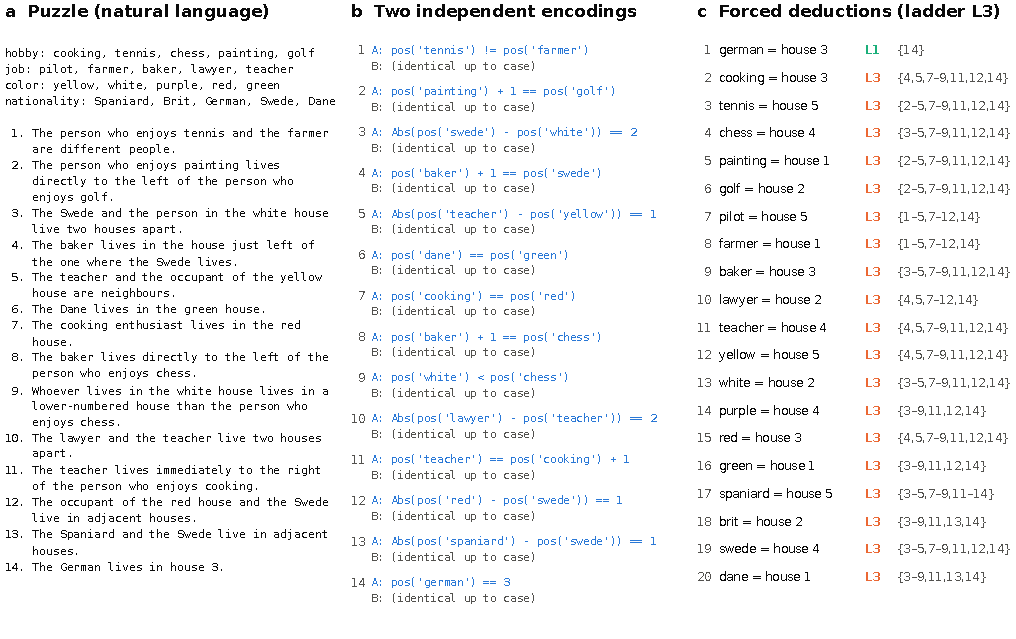
\includegraphics[width=\textwidth]{../figures/fig1_example.pdf}
\caption{One zebra puzzle through the pipeline. (a) The text given to the encoders. (b) The two Sonnet encodings in the position DSL; three clues are written differently and z3 proves $A \oplus B$ unsatisfiable. (c) Every fact of the solution in the order the ladder derives it, the strongest rule needed so far, and a minimal set of clues that forces it. The puzzle is L3: after one unit-propagation step every further fact needs failed-literal probing, and most explanations need 8--13 of the 14 clues.}
\label{fig:example}
\end{figure*}

\begin{figure}[t]
\centering
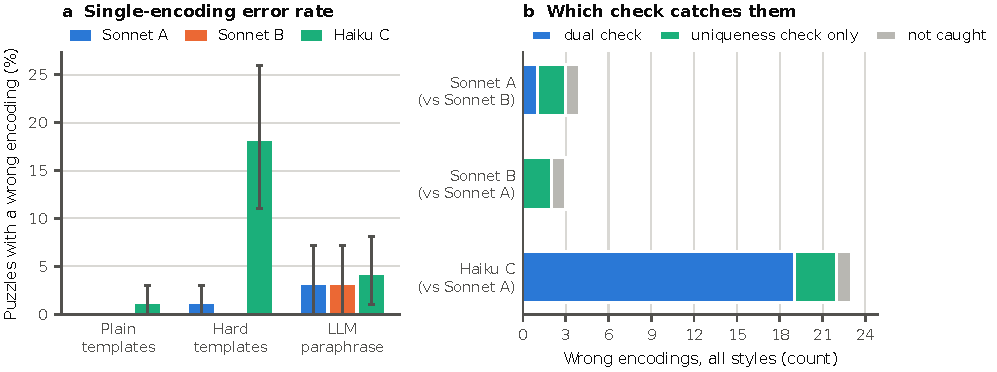
\includegraphics[width=\columnwidth]{../figures/fig2_faithfulness.pdf}
\caption{E1. (a) Share of puzzles with a wrong single encoding, with 95\% bootstrap intervals. (b) For each encoder, how its wrong encodings were detected: by disagreement with its partner encoding, or only because the wrongly encoded puzzle no longer had a unique solution. No wrong encoding escaped both checks.}
\label{fig:e1}
\end{figure}

\paragraph{Detection.} The dual check flagged every puzzle on which exactly one encoder of a pair was wrong. It missed the errors that both encoders shared: on paraphrased text the two Sonnet encodings disagreed on no puzzle at all, although both were wrong on the same 7. Each of those wrong encodings, however, made the encoded puzzle lose its unique solution, so the uniqueness check rejected it. Across all 299 puzzles and all three encoders, no wrong encoding passed both checks (Figure~\ref{fig:e1}b). Uniqueness works as a second detector because a minimal puzzle has no slack: changing the meaning of one clue almost always either removes the intended solution or admits a second one.

\paragraph{Audit.}\label{sec:audit} We read every clue-level error by hand (\texttt{results/e1/audit.md}). There were four groups.
(i) \emph{An ambiguous template of our own} (\EOneTaxTooStrong clue encodings per encoder): ``At least one house separates X and Y'' was generated for ``X and Y are not neighbours'' ($|p_X-p_Y|\neq1$, which allows the same house), and all three encoders read it as $|p_X-p_Y|\ge2$. Their reading is the natural one; the template is wrong. Because the clue is still true of the solution, no answer changed, and neither check can see the error; only the formal ground truth revealed it.
(ii) \emph{Counting from the right}: ``the fourth house from the right'' encoded as house~4 (Haiku 5 clues, Sonnet~B 1).
(iii) \emph{Direction flips}: ``the left-hand neighbour of the German drinks juice'' encoded with the German on the left (2 clues).
(iv) \emph{Paraphrase drift}: Sonnet, asked to keep the meaning exactly, rewrote ``exactly one house between X and Y'' as ``two houses separate X and Y'' in 7 puzzles. The encoders then encoded what the text said. This is an error of the text, not of the encoding, and dual encoding by construction cannot catch it.

\subsection{E2: LLM-written puzzles without and with the loop}

Sonnet's puzzles were almost always valid (Table~\ref{tab:e2}): \ETwoValid of \ETwoN parsed, had a unique solution equal to the stated one, and were fair. One Sudoku had a stated solution different from its true unique solution, and one Futoshiki had several solutions; one round of solver feedback repaired both (\ETwoValidRepair of \ETwoN). The zebra puzzles' two encodings never disagreed.

The puzzles were, however, easy and redundant (Figure~\ref{fig:e2}). All 20 Sudoku had exactly 30 givens and were solved by unit propagation alone; half of the Killer puzzles were L1. On average \ETwoSudokuRed of a Sudoku's givens, \ETwoKillerRed of a Killer puzzle's clues and \ETwoFutoshikiRed of a Futoshiki puzzle's clues could each be removed without losing uniqueness; for zebra puzzles the figure was \ETwoZebraRed. Minimising the LLM puzzles with the solver raised their level (Sudoku: \ETwoSudokuMinLC of 20 reached L3; zebra: \ETwoZebraMinLC of 40). The 20 Sudoku used only \ETwoSudokuMasks distinct layouts of givens; \ETwoSudokuWikiMask used the layout of the example puzzle on the English Wikipedia Sudoku page and \ETwoSudokuWikiSame reproduced that puzzle exactly. LLM-written puzzles are thus valid but not a good source of hard or novel instances, and copying is a real risk for benchmarks built this way.

\begin{table*}[t]
\centering
\caption{E2. Validity, level and redundancy of 100 puzzles written by Sonnet. ``Valid'' = parses, unique, matches the stated solution and fair (L1--L3). Levels are given as L1/L2/L3 counts before and after solver minimisation.}
\label{tab:e2}
\small
\begin{tabular}{lrrrrrccrc}
\toprule
Family & $n$ & unique & as stated & valid & after repair & levels (LLM) & levels (min.) & redundancy & clues \\
\midrule
\rows{e2_rows}
\bottomrule
\end{tabular}
\end{table*}

\begin{figure}[t]
\centering
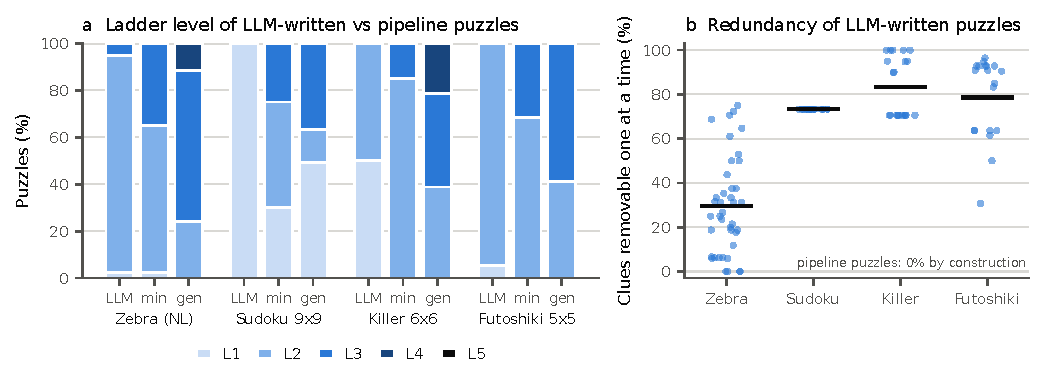
\includegraphics[width=\columnwidth]{../figures/fig3_validity.pdf}
\caption{E2. (a) Ladder levels of the LLM-written puzzles, of the same puzzles after solver minimisation, and of the pipeline's own bank. (b) Fraction of clues that can each be removed without losing uniqueness; the pipeline's puzzles have none by construction.}
\label{fig:e2}
\end{figure}

\subsection{E3: the ladder, solver effort and LLM accuracy}

\paragraph{Ladder versus solver metrics.} Within every family the ladder level tracks solver effort and explanation size (Figure~\ref{fig:metrics}, Table~\ref{tab:rho}). The Spearman correlation of level with MiniSat conflicts was \RhoZebraConflicts (zebra), \RhoSudokuConflicts (Sudoku), \RhoKillerConflicts (Killer) and \RhoFutoshikiConflicts (Futoshiki); with the share of variables fixed by unit propagation it was between \RhoSudokuUpClosure and \RhoZebraUpClosure. The level is not a proxy for the number of clues: in Sudoku the correlation with the number of givens was \RhoSudokuNClues, and in the other families harder puzzles had \emph{fewer} clues. Mean explanation size rises with level, so harder puzzles are also those in which each fact depends on more clues at once.

\begin{figure*}[t]
\centering
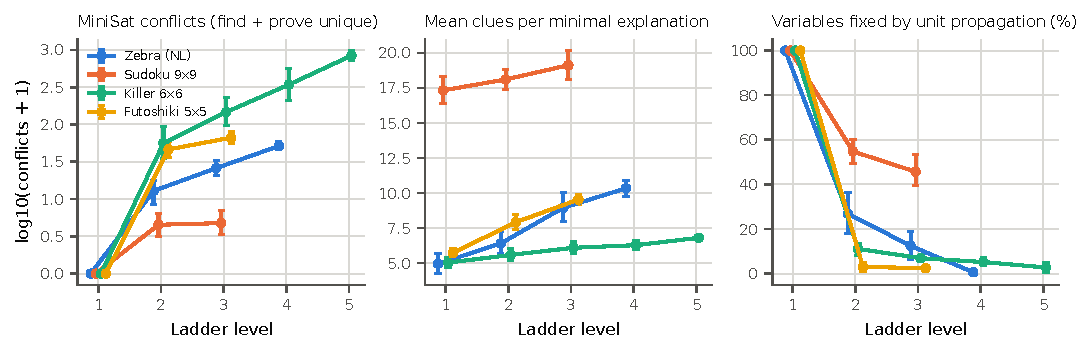
\includegraphics[width=\textwidth]{../figures/fig4_ladder_metrics.pdf}
\caption{E3. Solver-side metrics by ladder level for the 116 selected puzzles (means with 95\% bootstrap intervals). L1 cells of zebra, Killer and Futoshiki contain augmented puzzles.}
\label{fig:metrics}
\end{figure*}

\begin{table*}[t]
\centering
\caption{E3. Spearman correlation of ladder level with solver metrics, with 95\% bootstrap intervals.}
\label{tab:rho}
\small
\setlength{\tabcolsep}{3pt}
\begin{tabular}{lcccc}
\toprule
Metric & Zebra & Sudoku & Killer & Futoshiki \\
\midrule
\rows{e3rho_rows}
\bottomrule
\end{tabular}
\end{table*}

\paragraph{Ladder versus LLM accuracy.} Table~\ref{tab:acc} and Figure~\ref{fig:acc} give the exact-solution rates. Every model solved every zebra puzzle at every level, including the 8 L4 puzzles. Opus solved all \EThreeN puzzles; Sonnet missed one L5 Killer puzzle (with 35 of 36 cells right). Only Haiku made more than isolated errors, and mostly on Sudoku (\EThreeSudokuHaiku\% exact). Haiku's Sudoku accuracy fell from 6 of 8 at L1 and L2 to 3 of 8 at L3, but this drop needs care: \EThreeSudokuHaikuUnans of its 24 Sudoku items were left unanswered, 5 of them L3, and 5 of the 6 came from one call that gave up on its whole batch of five. Among the items Haiku did answer, it solved \EThreeSudokuHaikuAnsLA at L1, \EThreeSudokuHaikuAnsLB at L2 and \EThreeSudokuHaikuAnsLC at L3. Whether giving up is itself a sign of difficulty cannot be separated here from the batch it happened in.

Formally, on the family--model cells that are not at ceiling (Sudoku, Killer and Futoshiki for Haiku and Sonnet; $n=\LogitN$), the logistic slope of exact solution on level was \LogitLevel (95\% cluster-bootstrap interval \LogitLevelLo{} to \LogitLevelHi; $p=\LogitLevelP$). A linear mixed model of cell accuracy over all 348 attempts gave a level slope of \MixedLevel{} per level (SE \MixedLevelSE, $p=\MixedLevelP$). Adding the level to a model with MiniSat conflicts, explanation size and number of clues lowered the AIC from \AICMetrics{} to \AICMetricsLevel{}, so the ladder carries some information that raw solver effort does not, but the evidence is weak. The honest summary is that for current models these puzzle sizes are mostly too easy for the ladder to predict accuracy: it predicts solver effort well and LLM failure poorly, because there are few failures to predict.

\begin{table}[t]
\centering
\caption{E3. Exact solutions (\%) with 95\% bootstrap intervals, all levels pooled. Unanswered items count as wrong (Haiku: 6 Sudoku and 2 Futoshiki items).}
\label{tab:acc}
\small
\setlength{\tabcolsep}{3pt}
\begin{tabular}{lccc}
\toprule
Family & Haiku & Sonnet & Opus \\
\midrule
\rows{e3acc_rows}
\bottomrule
\end{tabular}
\end{table}

\begin{figure*}[t]
\centering
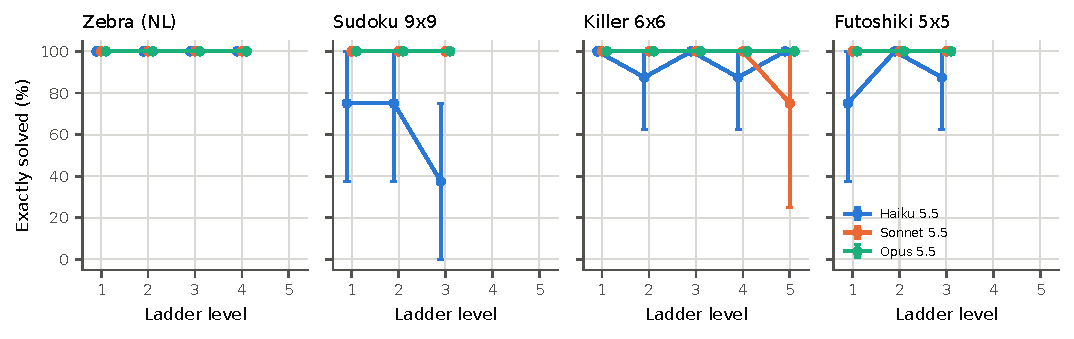
\includegraphics[width=\textwidth]{../figures/fig5_ladder_accuracy.pdf}
\caption{E3. Exact-solution rate by ladder level, family and model (95\% bootstrap intervals; 8 puzzles per cell except Killer L5 with 4). Sudoku has no L4--L5 cells because none occurred among 9{,}500 generated puzzles; Futoshiki $5{\times}5$ has none above L3.}
\label{fig:acc}
\end{figure*}

\subsection{E4: evolving fair puzzles against a solver}

\paragraph{Zebra.} A pilot on $5{\times}4$ zebra puzzles and the main run on $6{\times}6$ zebra puzzles both ended without a single training-solver error. Over \EFourZebraGens evaluated generations the $6{\times}6$ run produced \EFourZebraIndiv fair individuals (\EFourZebraLB at L2, \EFourZebraLC at L3) from \EFourZebraAccepted accepted of \EFourZebraProposals proposed edits, and Haiku solved every one of \EFourZebraEvals evaluations exactly; the pilot (\EFourPilotIndiv individuals, \EFourPilotEvals evaluations) was the same. With no error, fitness is zero everywhere and selection has nothing to act on (Figure~\ref{fig:evo}a). Fresh calls of all three models also solved every initial and final individual (Figure~\ref{fig:evo}b). Fair zebra puzzles of this size are therefore not hard for Haiku, and we stopped the zebra runs.

\paragraph{Sudoku.} PENDING


\begin{figure*}[t]
\centering
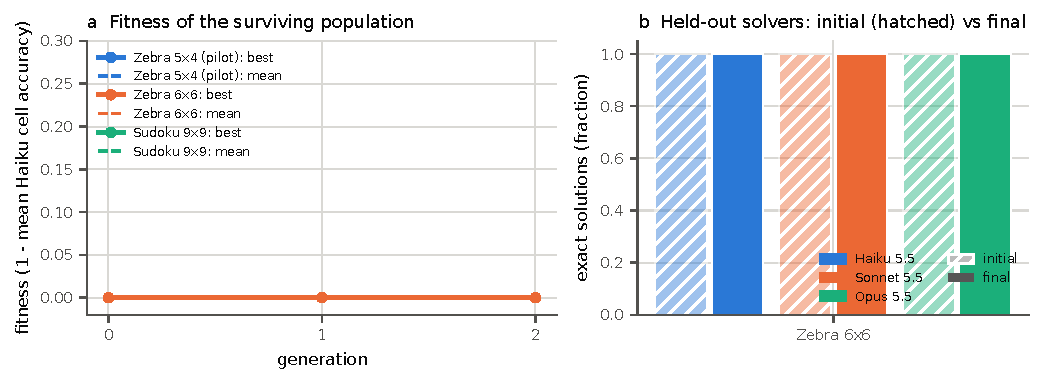
\includegraphics[width=0.85\textwidth]{../figures/fig6_evolution.pdf}
\caption{E4. (a) Best and mean fitness of the surviving population per generation (fitness = 1 $-$ mean Haiku cell accuracy over all evaluations of an individual). (b) Exact-solution rate of fresh solver calls on the initial (hatched) and final populations.}
\label{fig:evo}
\end{figure*}

\subsection{E5: genres invented by an LLM}

All \EFiveGenres genres that Sonnet wrote compiled in the sandbox, and the pipeline built and certified 12 minimal unique instances of each (Table~\ref{tab:e5}). Most genres are Latin squares with a new clue type: parity and sums of neighbours, sums of mirrored cells, cells a knight's move apart that must differ, or bans on neighbouring digits two apart. Their certified instances are mostly L3. The genre we find most interesting is \emph{Median Line Latin} (Figure~\ref{fig:gallery}e): a $5{\times}5$ Latin square whose clues either give the sum of two or three neighbouring cells or state that the middle of three consecutive cells has a value strictly between the other two. Eight of its 12 instances need two-level lookahead (L4) with about 7 clues, the deepest of all genres. The ``median'' clue is weak on its own (it rules out only the two extreme values of the middle cell) but combines with the Latin rules into long chains, which is what the ladder detects. All three models nevertheless solved all four L4 instances of this genre that we gave them (\EFiveSolveExact of \EFiveSolveN attempts).

\begin{table}[t]
\centering
\caption{E5. Genres invented by Sonnet: certified instances and their ladder levels.}
\label{tab:e5}
\small
\setlength{\tabcolsep}{3pt}
\begin{tabular}{lcrrrrrr}
\toprule
Genre & certified & L1 & L2 & L3 & L4 & L5 & clues \\
\midrule
\rows{e5_rows}
\bottomrule
\end{tabular}
\end{table}

\begin{figure*}[t]
\centering
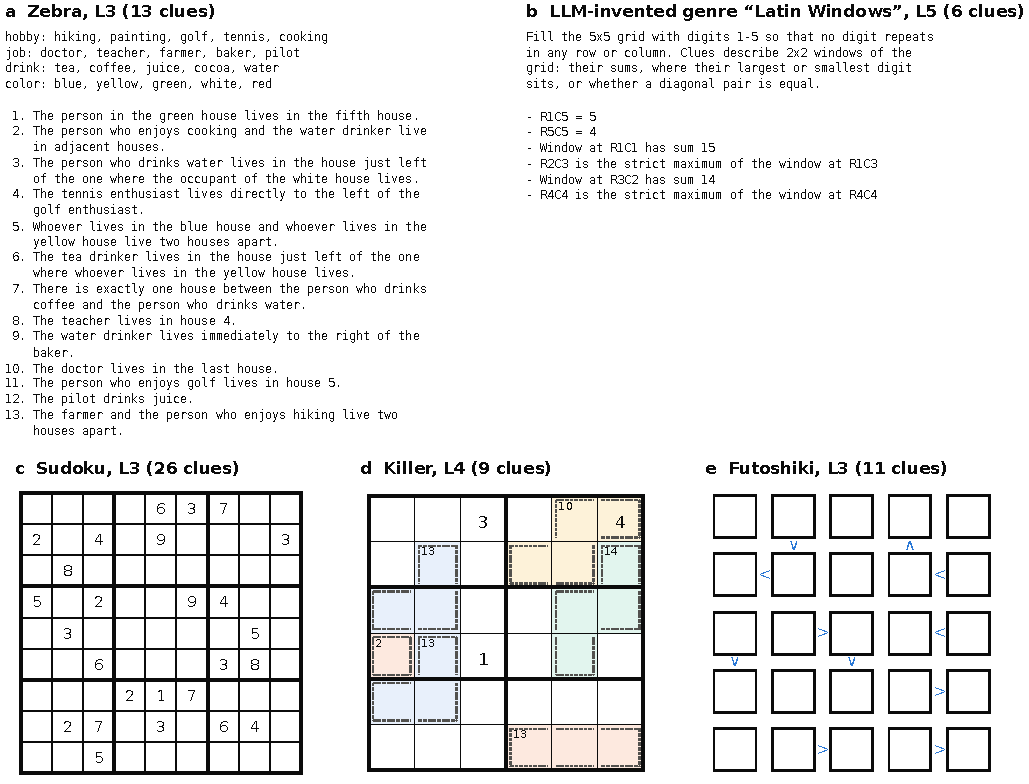
\includegraphics[width=0.92\textwidth]{../figures/fig7_gallery.pdf}
\caption{Gallery of certified puzzles from the benchmark: (a) zebra, (b) Sudoku, (c) Killer (cages with sums), (d) Futoshiki, (e) the LLM-invented genre Median Line Latin. Levels are ladder levels; every puzzle is minimal and unique.}
\label{fig:gallery}
\end{figure*}

\section{Discussion}
\label{sec:discussion}

\paragraph{What the solver loop buys.} The loop turns a model's claim (``this puzzle has one answer'') into a certificate, but the certificate covers the encoding, not the text. Our results suggest three practical rules. First, the translation from text to constraints is reliable when the text is regular: on template text no encoder made any error. Second, dual encoding catches independent misreadings, which are what a second model run is good at, but not errors that two runs share, and two runs of the same model share a great deal: the two Sonnet encoders agreed on every paraphrased puzzle, including the seven they both got wrong. Third, uniqueness is a strong and cheap second check for minimal puzzles, because a minimal puzzle has no slack: a misread clue almost always removes the intended solution or lets in another. The combination caught every wrong encoding we observed. What it cannot catch is an error that leaves the puzzle unique with the same answer, such as our own ambiguous template; such errors do not change the answer but do mean the text says something other than the certificate, which matters if the puzzle is used to teach or to explain.

\paragraph{LLM-written puzzles.} Sonnet's puzzles were valid far more often than we expected, and one round of solver feedback fixed the rest. The problem is not validity but quality: they are easy, padded with redundant clues, and in Sudoku they reuse a famous layout. A solver that minimises and grades the puzzle fixes the first two; the third is a warning for anyone who builds evaluation sets by asking a model for puzzles.

\paragraph{The ladder.} Five nested propagation engines give a level that is cheap to compute, interpretable in solving terms, and closely related to solver effort and to the size of minimal explanations in every family. It does not, at these sizes, predict whether current LLMs succeed, because they almost always do. The exception is the smallest model on $9{\times}9$ Sudoku, where failures, and especially give-ups, concentrate in the higher levels, though our data cannot separate level from batch effects there. A ladder whose top levels are rare in random generation (no Sudoku above L3 in 9{,}500) is also a ladder whose top levels must be searched for, which is what E4 attempts.

\paragraph{Fair but hard.} We did not find fair zebra puzzles that Haiku fails. This is a null result at our scale (two runs, at most three generations, 8 individuals) and it does not show that such puzzles do not exist; but the space we searched, all unique L1--L3 puzzles of size up to $6{\times}6$, was solved without error in \EFourZebraEvals of \EFourZebraEvals attempts. Larger instances, other genres, or fitness based on solving cost rather than errors may behave differently.

\section{Limitations}
\label{sec:limitations}

\begin{itemize}[leftmargin=1.2em,itemsep=1pt,topsep=2pt]
\item \emph{How the models were called.} No API key was available, so every call was a fresh Claude Code subagent with no shared context (Section~\ref{sec:llmcalls}). Temperature and reasoning settings were not under our control, model versions are identified by alias, and the workers had a general system prompt we did not write. The audit of tool calls (\NAudited of \NCalls calls matched to transcripts) found no code execution; \NForbidden calls made one extra status or messaging call with no puzzle content (one edited its own output file), and \NExtraWrite wrote their output in several steps. Calls with extra tool use were kept.
\item \emph{Scale.} The study is small: 299 puzzles in E1, 100 in E2, 116 in E3, three evolution runs. Rates near zero have wide intervals, and E3 has 8 puzzles per cell (4 for Killer L5).
\item \emph{Batching.} Several items share a call. Items in a call are not independent, and a call that gives up affects all its items (one Haiku Sudoku call left five items unanswered, which we score as wrong).
\item \emph{Augmented L1 puzzles.} L1 cells of three families were filled by adding redundant clues to minimal puzzles, so they differ from the other cells in clue count and redundancy.
\item \emph{Ground truth in E1} comes from our generator; one of its templates was ambiguous, which we report as a finding rather than an encoder error.
\item \emph{Cost} is estimated from total token counts with a conservative split between input and output and list prices without caching; real costs would be lower.
\item \emph{Ladder.} The ladder is defined on one CNF encoding; a different encoding (for example with auxiliary variables) would change what unit propagation can do, and humans' notion of difficulty is not modelled.
\end{itemize}


\section*{Data and code availability}
All code, configuration, prompts, task files, model outputs, intermediate results and figures are in the project repository,\\ \url{https://github.com/sarabehnamian/Puzzle-generation-with-guaranteed-uniqueness}.\\ The benchmark (\texttt{benchmark/}) contains the certified puzzles with their solutions, ladder levels, solver metrics and minimal-core explanations, with a datasheet \citep{gebru2021datasheets}. Every number in this paper is written to \texttt{paper/numbers.tex} by \texttt{src/make\_numbers.py} from saved results. The reported results use \NCallsFinal Messages API calls with \TokensFinalM million tokens, which cost \$\CostFinal at list prices. Including the discarded batched solving run and a run affected by an answer-parsing bug that we fixed, the study made \NCalls calls with \TokensM million tokens for \$\CostUSD (exact token counts; see \texttt{results/cost\_summary.json} and \texttt{src/cost.py}).

\section*{Acknowledgements}
The experiments, analysis code and a first draft of this text were produced with the help of Claude Code (Anthropic); the author is responsible for the content.

\bibliographystyle{plainnat}
\bibliography{references}

\end{document}
